%\begin{frame}[standout]
%	\Huge \textsc{Goal Dependencies}
%\end{frame}

\begin{frame}{Oversubscription Planning and Goal Properties}
	\begin{center}
		\begin{tikzpicture}
			\node[] (el) at (0,0) {\Large Energy Limit};
			\node[] (el) at (0,-1) {
\includegraphics[scale=0.2]{images/battarie_low.png}};
		%\visible<3>{
		%\begin{tikzpicture}
		%	\node[] (i1) at (0,0) {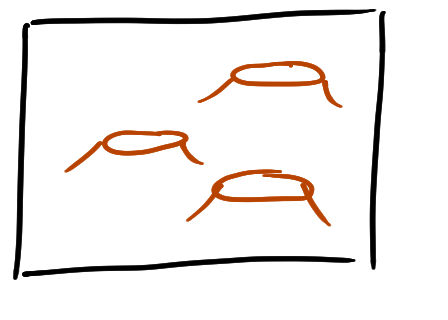
\includegraphics[scale=0.15]{images/image1.png}};
		%	\node[] (i2) at (3,0) {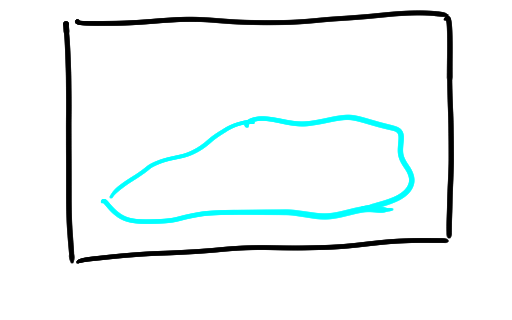
\includegraphics[scale=0.15]{images/image3.png}};
		%	\node[] (i3) at (6.2,0) {
\includegraphics[scale=0.15]{images/image2.png}};
		%	\node[] (and) at (1.4,0) {\Huge $\wedge$};
		%	\node[] (and) at (4.7,0) {\Huge $\vee$};
		%	\node[] (gd) at (3,-1.7) {\huge Goal Property};
		%
		%\end{tikzpicture}
		%}


			%\node[draw, fill=mLightBrown!30] (mugs1) at (5,0) {
			%	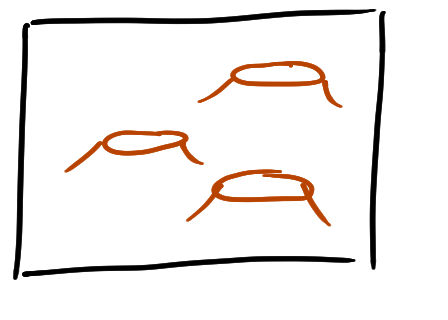
\includegraphics[scale=0.09]{images/image1.png} 
			%	
\includegraphics[scale=0.09]{images/image2.png}
			%};
			\node[draw, fill=mLightBrown!30] (mugs2) at (5,-1) {
				
\includegraphics[scale=0.09]{images/image2.png}
				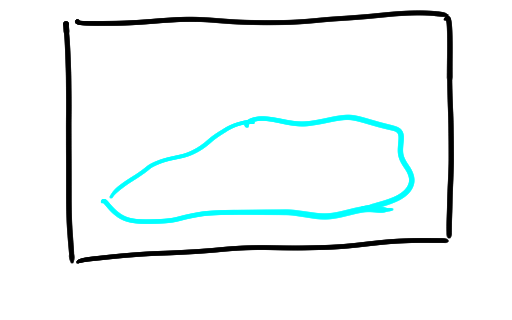
\includegraphics[scale=0.09]{images/image3.png} 
			};
		\end{tikzpicture}
	\end{center}


	\vspace*{0.3cm}
	\hrule
	\vspace*{0.5cm}
	\visible<2->{
	\large\textbf{$\plans$-Entailment}:\\
	\begin{center}
	\begin{tikzpicture}
		%\node[] (i1) at (0,0) {
		%	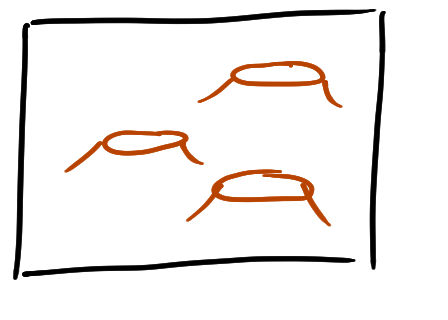
\includegraphics[scale=0.1]{images/image1.png} 
		%};
		%\node[] (i2) at (3,0) {
		%	
\includegraphics[scale=0.1]{images/image2.png}
		%};
		%\node[] (n1) at (3,0) {
		%	
\includegraphics[scale=0.1]{images/no.png} 
		%};
		%\node[] (i22) at (0,-1.8) {
		%	
\includegraphics[scale=0.1]{images/image2.png}
		%};
		%\node[] (i12) at (3,-1.8) {
		%	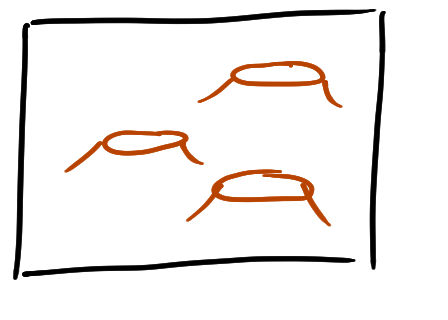
\includegraphics[scale=0.1]{images/image1.png}
		%};
		%\node[] (n2) at (3,-1.8) {
		%	
\includegraphics[scale=0.1]{images/no.png}
		%};

		%\draw[thick, ->] (i1) to (i2);
		%\draw[thick, ->] (i22) to (i12);

		\visible<2->{
		\node[] (i23) at (5,0) {
			
\includegraphics[scale=0.1]{images/image2.png} 
		};
		\node[] (i3) at (8,0) {
			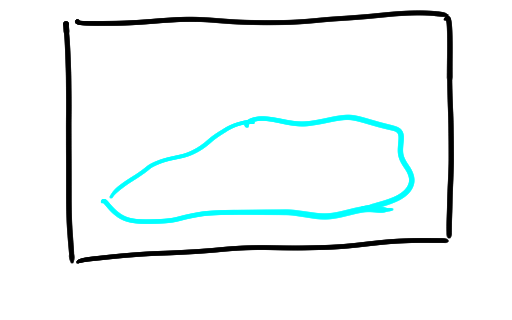
\includegraphics[scale=0.1]{images/image3.png}
		};
		\node[] (n3) at (8,0) {
			
\includegraphics[scale=0.1]{images/no.png} 
		};
		\node[] (i32) at (5,-1.8) {
			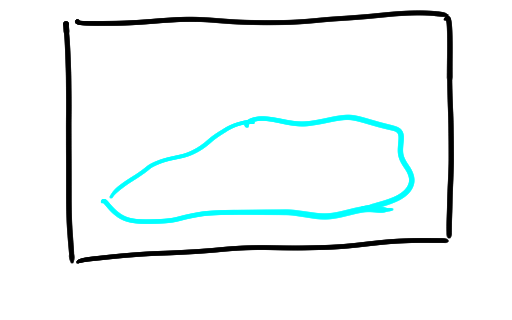
\includegraphics[scale=0.1]{images/image3.png}
		};
		\node[] (i24) at (8,-1.8) {
			
\includegraphics[scale=0.1]{images/image2.png}
		};
		\node[] (n4) at (8,-1.8) {
			
\includegraphics[scale=0.1]{images/no.png}
		};

		\draw[thick, ->] (i23) to (i3);
		\draw[thick, ->] (i32) to (i24);
		}
	\end{tikzpicture}
	}
	\end{center}

	
\end{frame}



